\section{Simulation of polymer viscosity distribution}
In this study, simulation of exposed polymer resist viscosity distribution is based on Monte-Carlo simulation of e-beam scattering in PMMA. The algorithm described in \cite{my_MEE} was used to simulate polymer main-chain scissions during the resist exposure in series of parallel lines. E-beam energy  was 20 keV, exposure current -- 0.03 nA per 1 cm of line, PMMA layer thickness -- 500 nm, line pitch -- 3 $\mu$m (Fig.~\ref{fig:sci_hist}).

\begin{figure}
	\begin{center}
		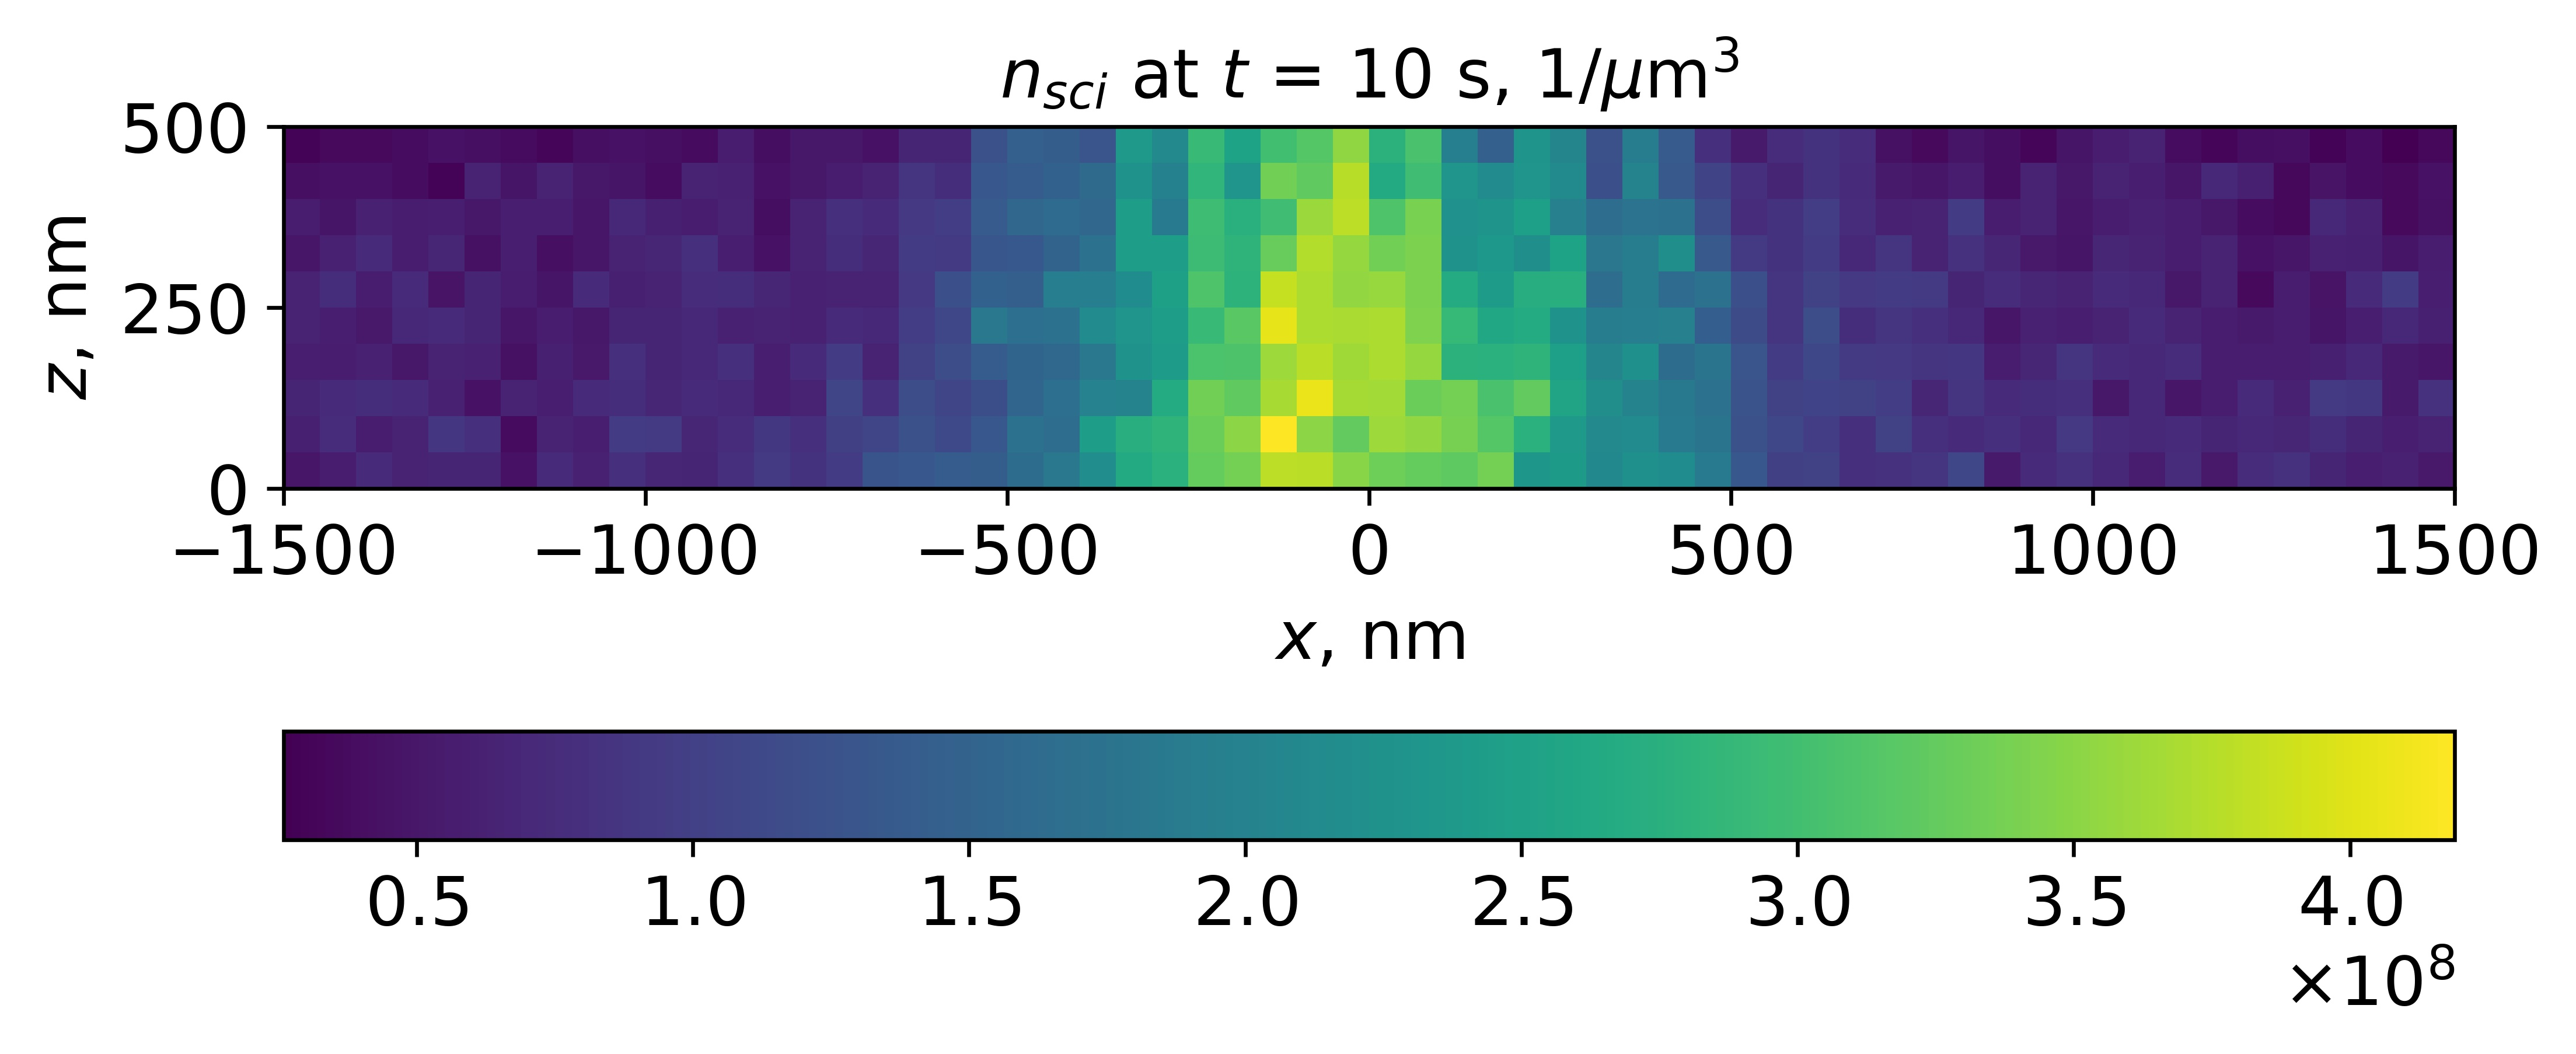
\includegraphics[width=0.7\linewidth]{sci_hist_10s_14_eng} \\
		\vspace{-3.7em} \hspace{-26em} a) \vspace{2.7em} \\
		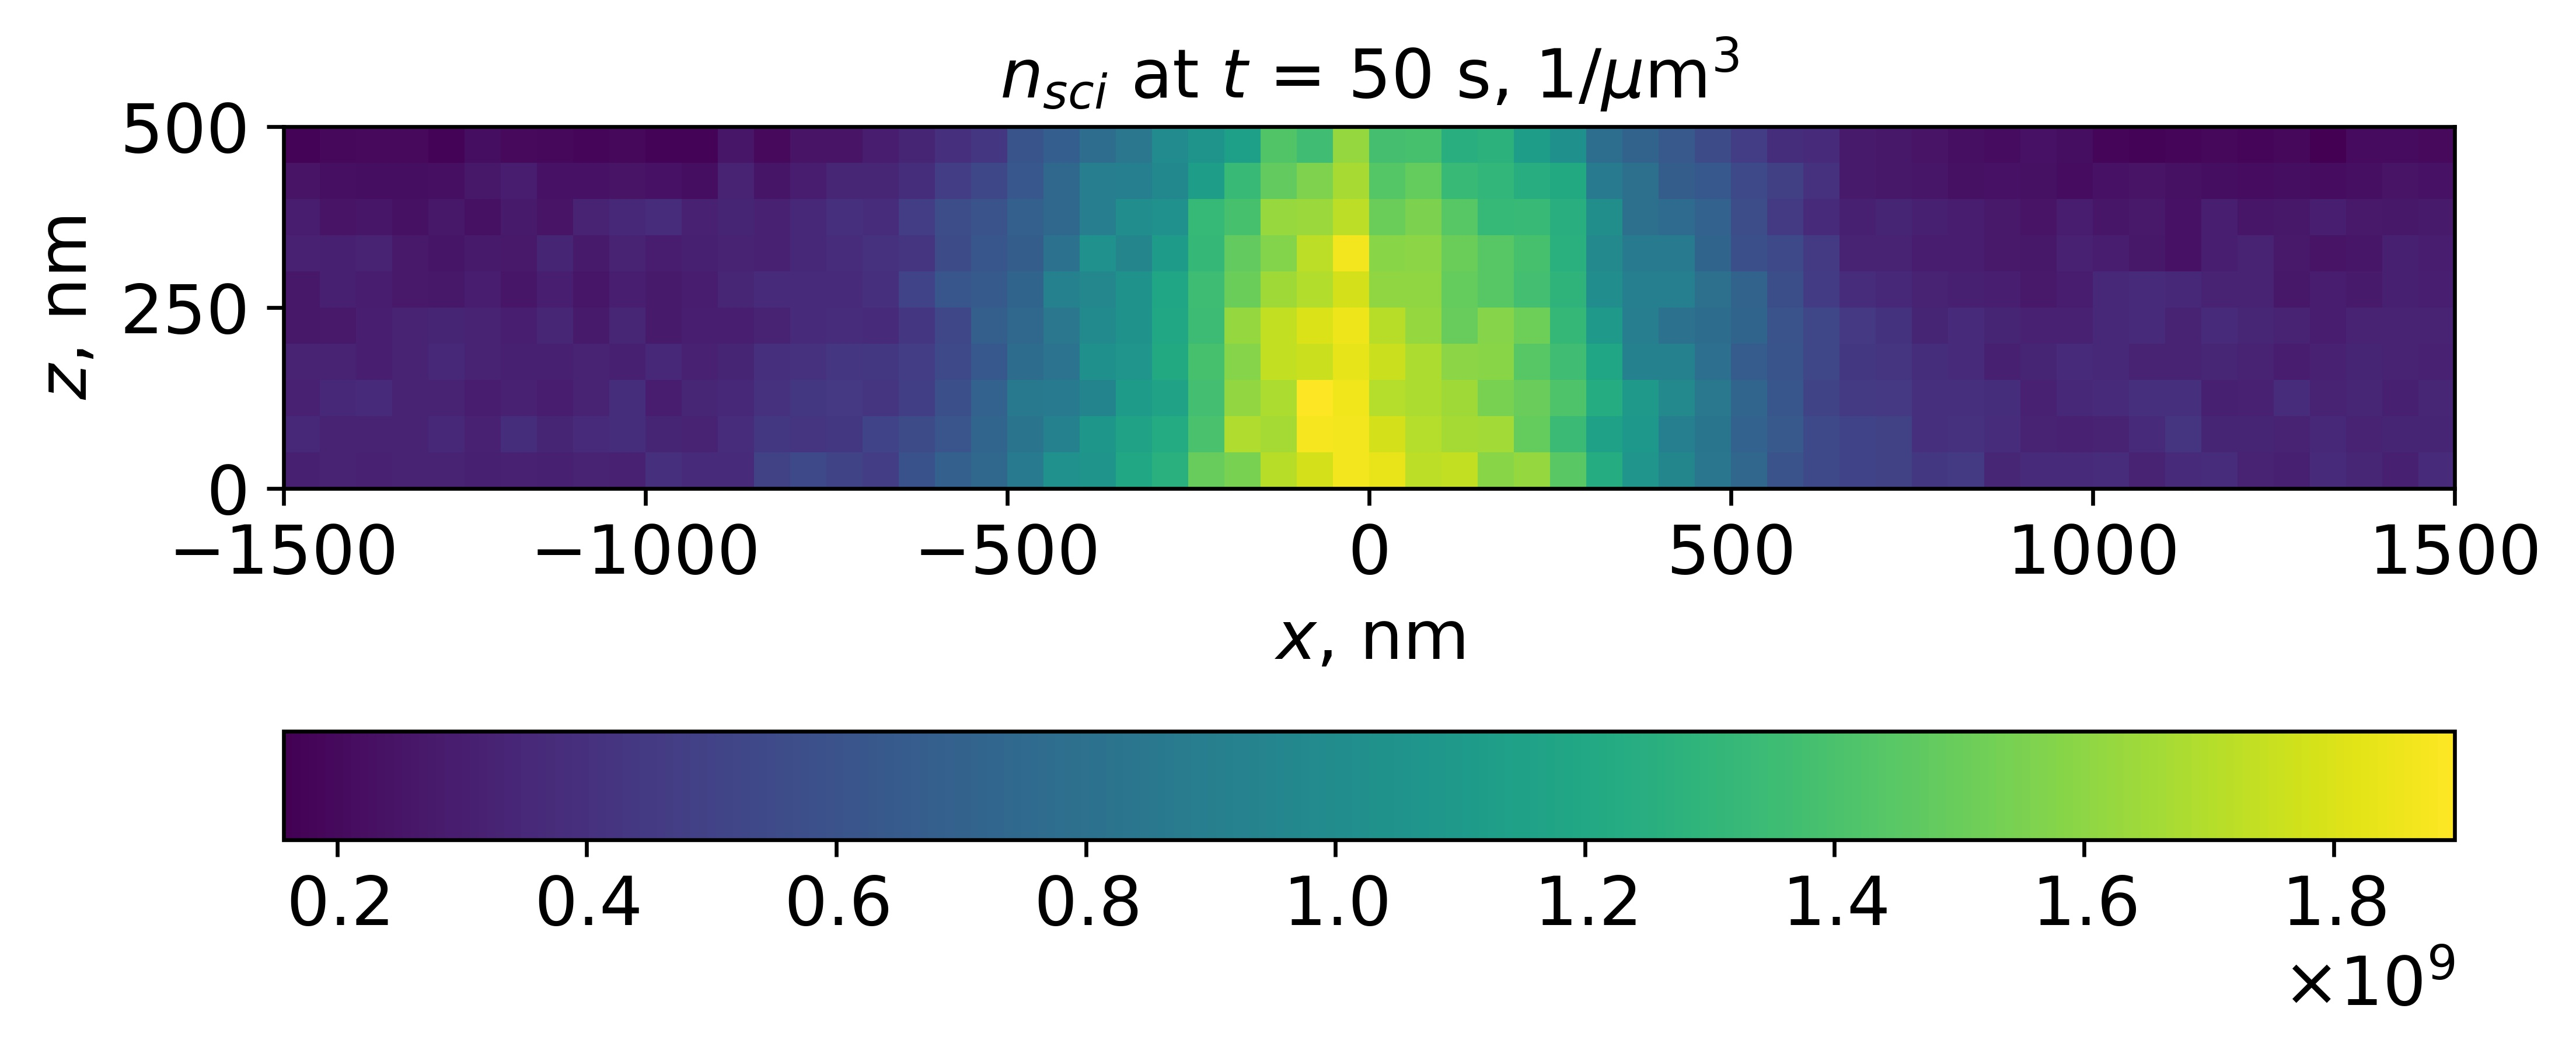
\includegraphics[width=0.7\linewidth]{sci_hist_50s_14_eng} \\
		\vspace{-3.7em} \hspace{-26em} b) \vspace{3.7em} \\
	\end{center}
	\vspace{-2.5em}
	\caption{Simulation of scission distribution in PMMA layer, obtained by the model described in~\cite{my_MEE} for exposure in series of parallel lines at 130~$^\circ$C. Line current is around 0.03 nA/cm, e-beam energy is 20 keV, PMMA layer thickness -- 500 nm, exposure time is 10 s (a) and  50 s (b).}
	\label{fig:sci_hist}
\end{figure}

Then PMMA layer was divided into 50 nm cells for the calculation of local depolymerization initiation constant $k_\mathrm{S}$ -- the number of PMMA main-chain scissions per monomer per 1 s. The number of monomers in each cell was determined from PMMA density and molar mass and comprised 894809.

Simulation of local $k_\mathrm{S}$ for each moment of exposure allowed to apply the kinetic approach for the simulation of polymer thermal depolymerization~\cite{Boyd_1}:

\begin{equation} \label{eq:moment_equation}
	\frac{d M_i}{d t}=k_\mathrm{S}(\frac{2}{i+1}-1) M_{i+1}+\frac{d M_0}{d t}-k_\mathrm{S} M_1 - \frac{i}{\gamma}(k_\mathrm{S} M_i+\frac{d M_{i-1}}{d t}) \quad(i \geq 1),
\end{equation}
where $1/\gamma$ -- average depolymerization zip length, $M_i$ -- moment of molecular weight distribution of $i$-th order:

\begin{equation}
	M_i=\sum_{n=2}^{\infty} n^i P_n.
\end{equation}

The solution of system~\ref{eq:moment_equation} proposed in~\cite{Boyd_3} is obtained for Schulz-Zimm polymer weight distribution~\cite{Schulz-Zimm_distribution}:

\begin{equation} \label{eq:Schulz-Zimm_distribution}
	P_n = C_0 n^z \exp (-n/y)
\end{equation}
where $P_n$ -- number of molecules with degree of polymerization equal to $n$, $C_0$ -- normalization factor. Parameter $z$ describes the width of distribution:

\begin{equation} \label{eq:Schulz-Zimm_1}
	M_w / M_N=(z+2) /(z+1),
\end{equation}
where $M_n$ and $M_w$ -- number average and weight average molecular weight, respectively, parameter $y$ is related to number average polymerization degree $x$:

\begin{equation} \label{eq:Schulz-Zimm_2}
	x=y(z+1).
\end{equation}

The higher moments of Schulz-Zimm distribution could be expressed by the equation

\begin{equation}
	M_i=M_1 \prod_{n=2}^i(z+n) y^{i-1},
\end{equation}
which allows to reduce the required nuber of equations in system~\ref{eq:moment_equation} to 3 (for three parameters of function~\ref{eq:Schulz-Zimm_distribution}) and then solve it numerically (see Appendix). This provides local $M_n$ and $M_w$ dependence on exposure time (Fig.~\ref{fig:Mn_Mw_tau}), which allows to determine the local polymer viscosity distribution at any given moment (Fig.~\ref{fig:Mn_hist}). Required average depolymerization zip length was obtained by exponential fit of values provided by Mita~\cite{Mita_PMMA_zip_lengths_T} for PMMA in case of depolymerization termination or chain transfer at the end of molecule. The result of PMMA molecular weight simulation for different exposure moments is shown in Fig.~\ref{fig:Mn_hist}.


\begin{figure}
	\begin{minipage}{0.48\textwidth}
		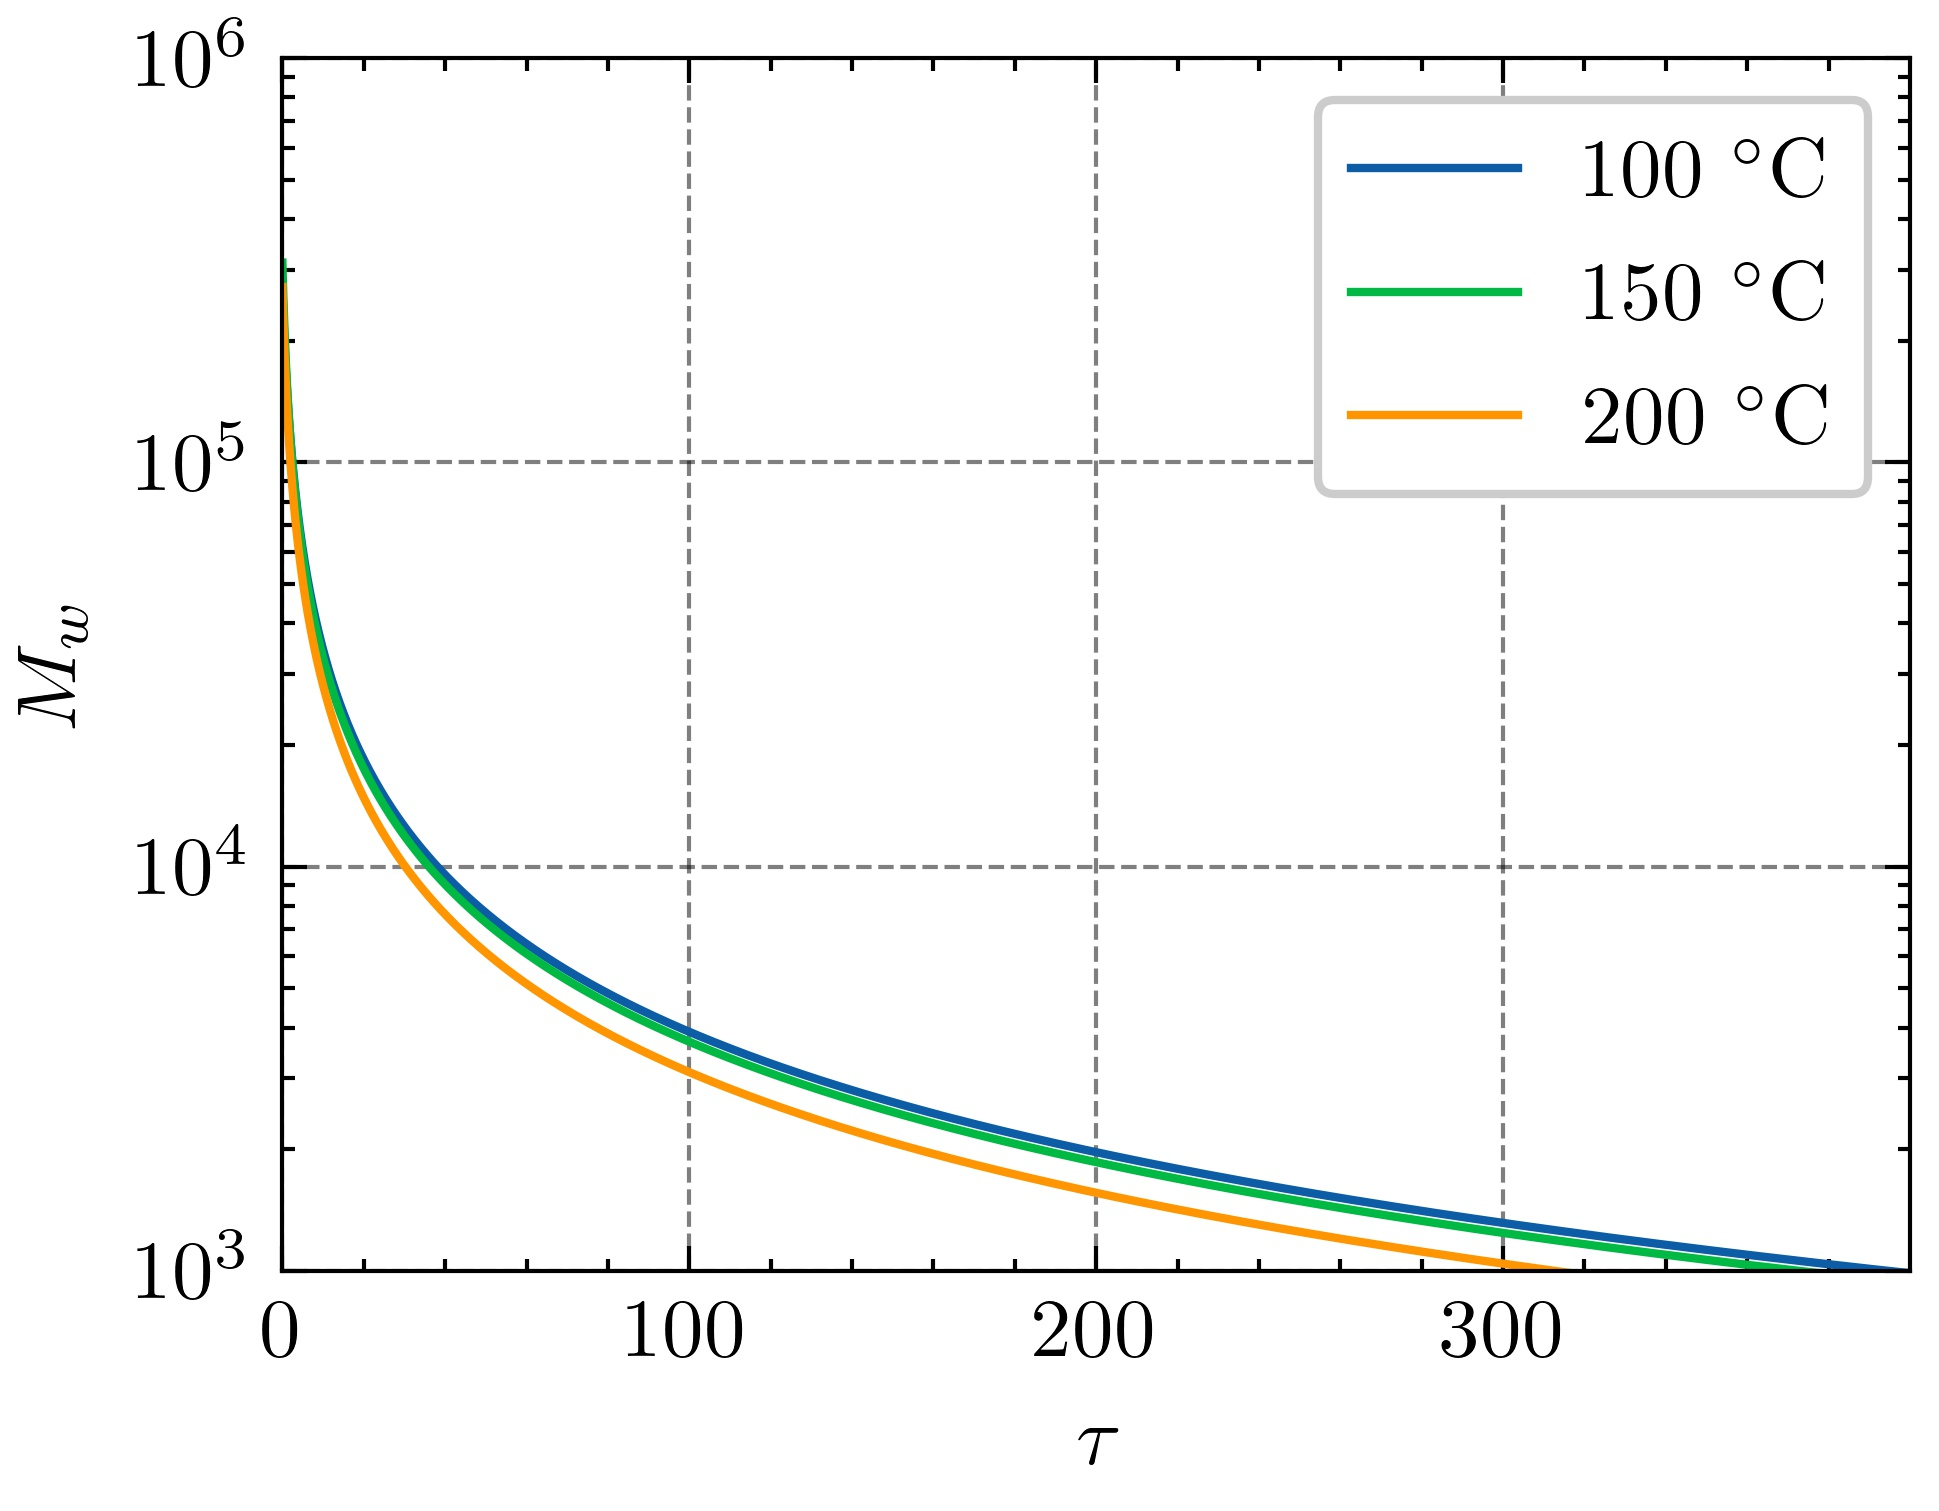
\includegraphics[width=\linewidth]{Mn_tau_100_150_200} \\
		\vspace{-14em} \\ \hspace{0em} a) \\ \vspace{14em}
	\end{minipage}
	\begin{minipage}{0.48\textwidth}
		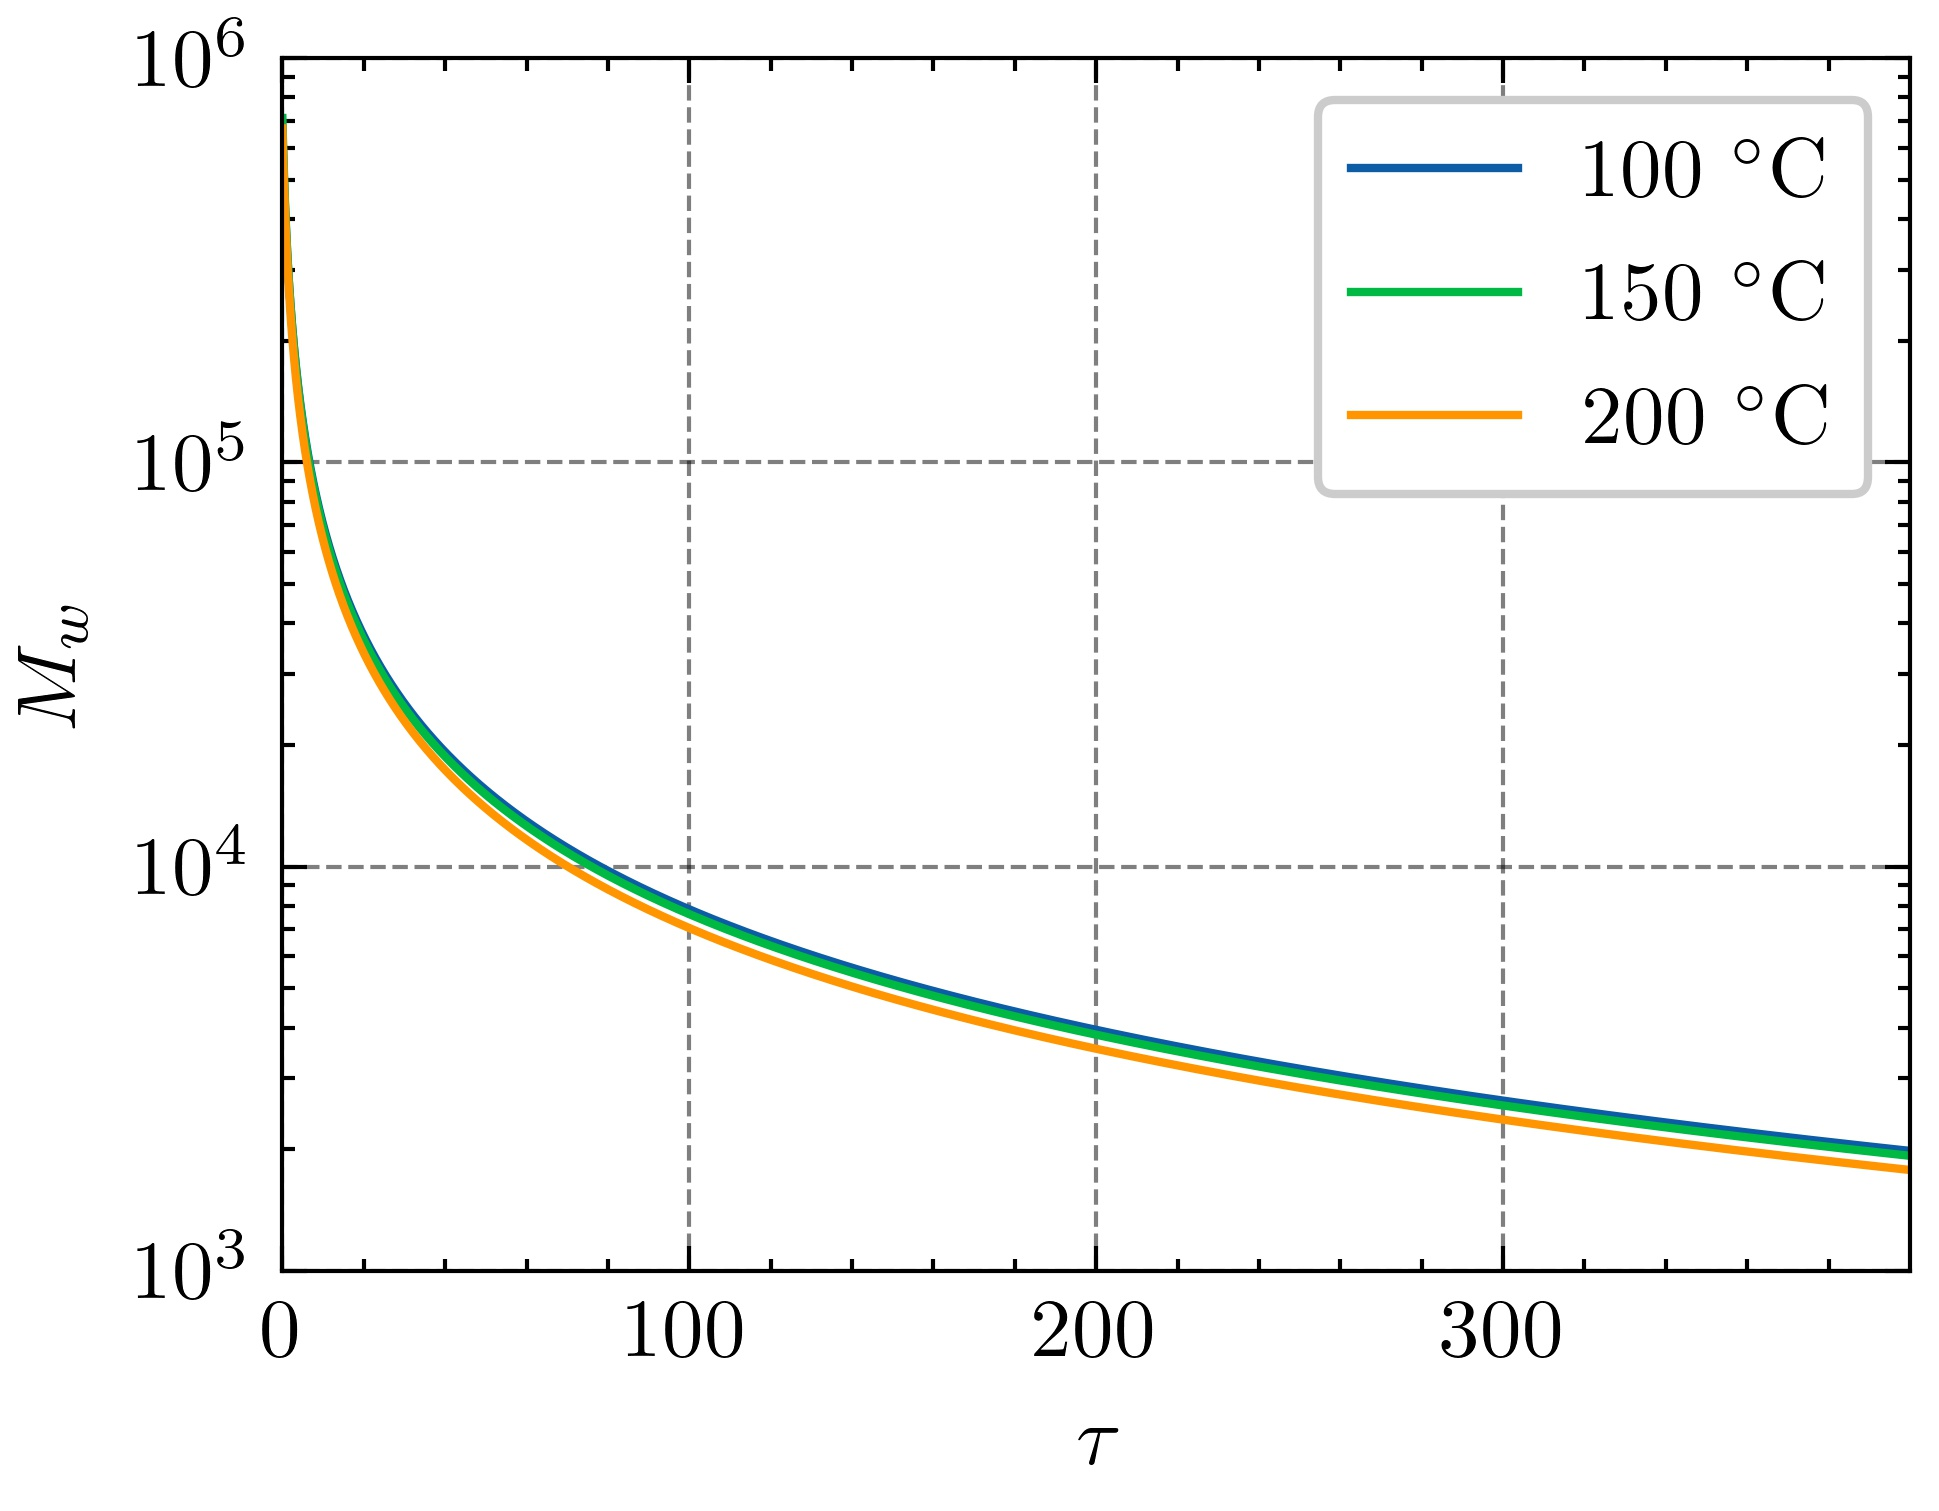
\includegraphics[width=\linewidth]{Mw_tau_100_150_200} \\
		\vspace{-14em} \\ \hspace{-0.1em} b) \\ \vspace{14em}
	\end{minipage}
	\vspace{-4em}
	\caption{$M_n$ and $M_w$ dependence on $\tau$ obtained by approach provided in~\cite{Boyd_3}.}
	\label{fig:Mn_Mw_tau}
\end{figure}

\begin{figure}[h]
	\begin{center}
		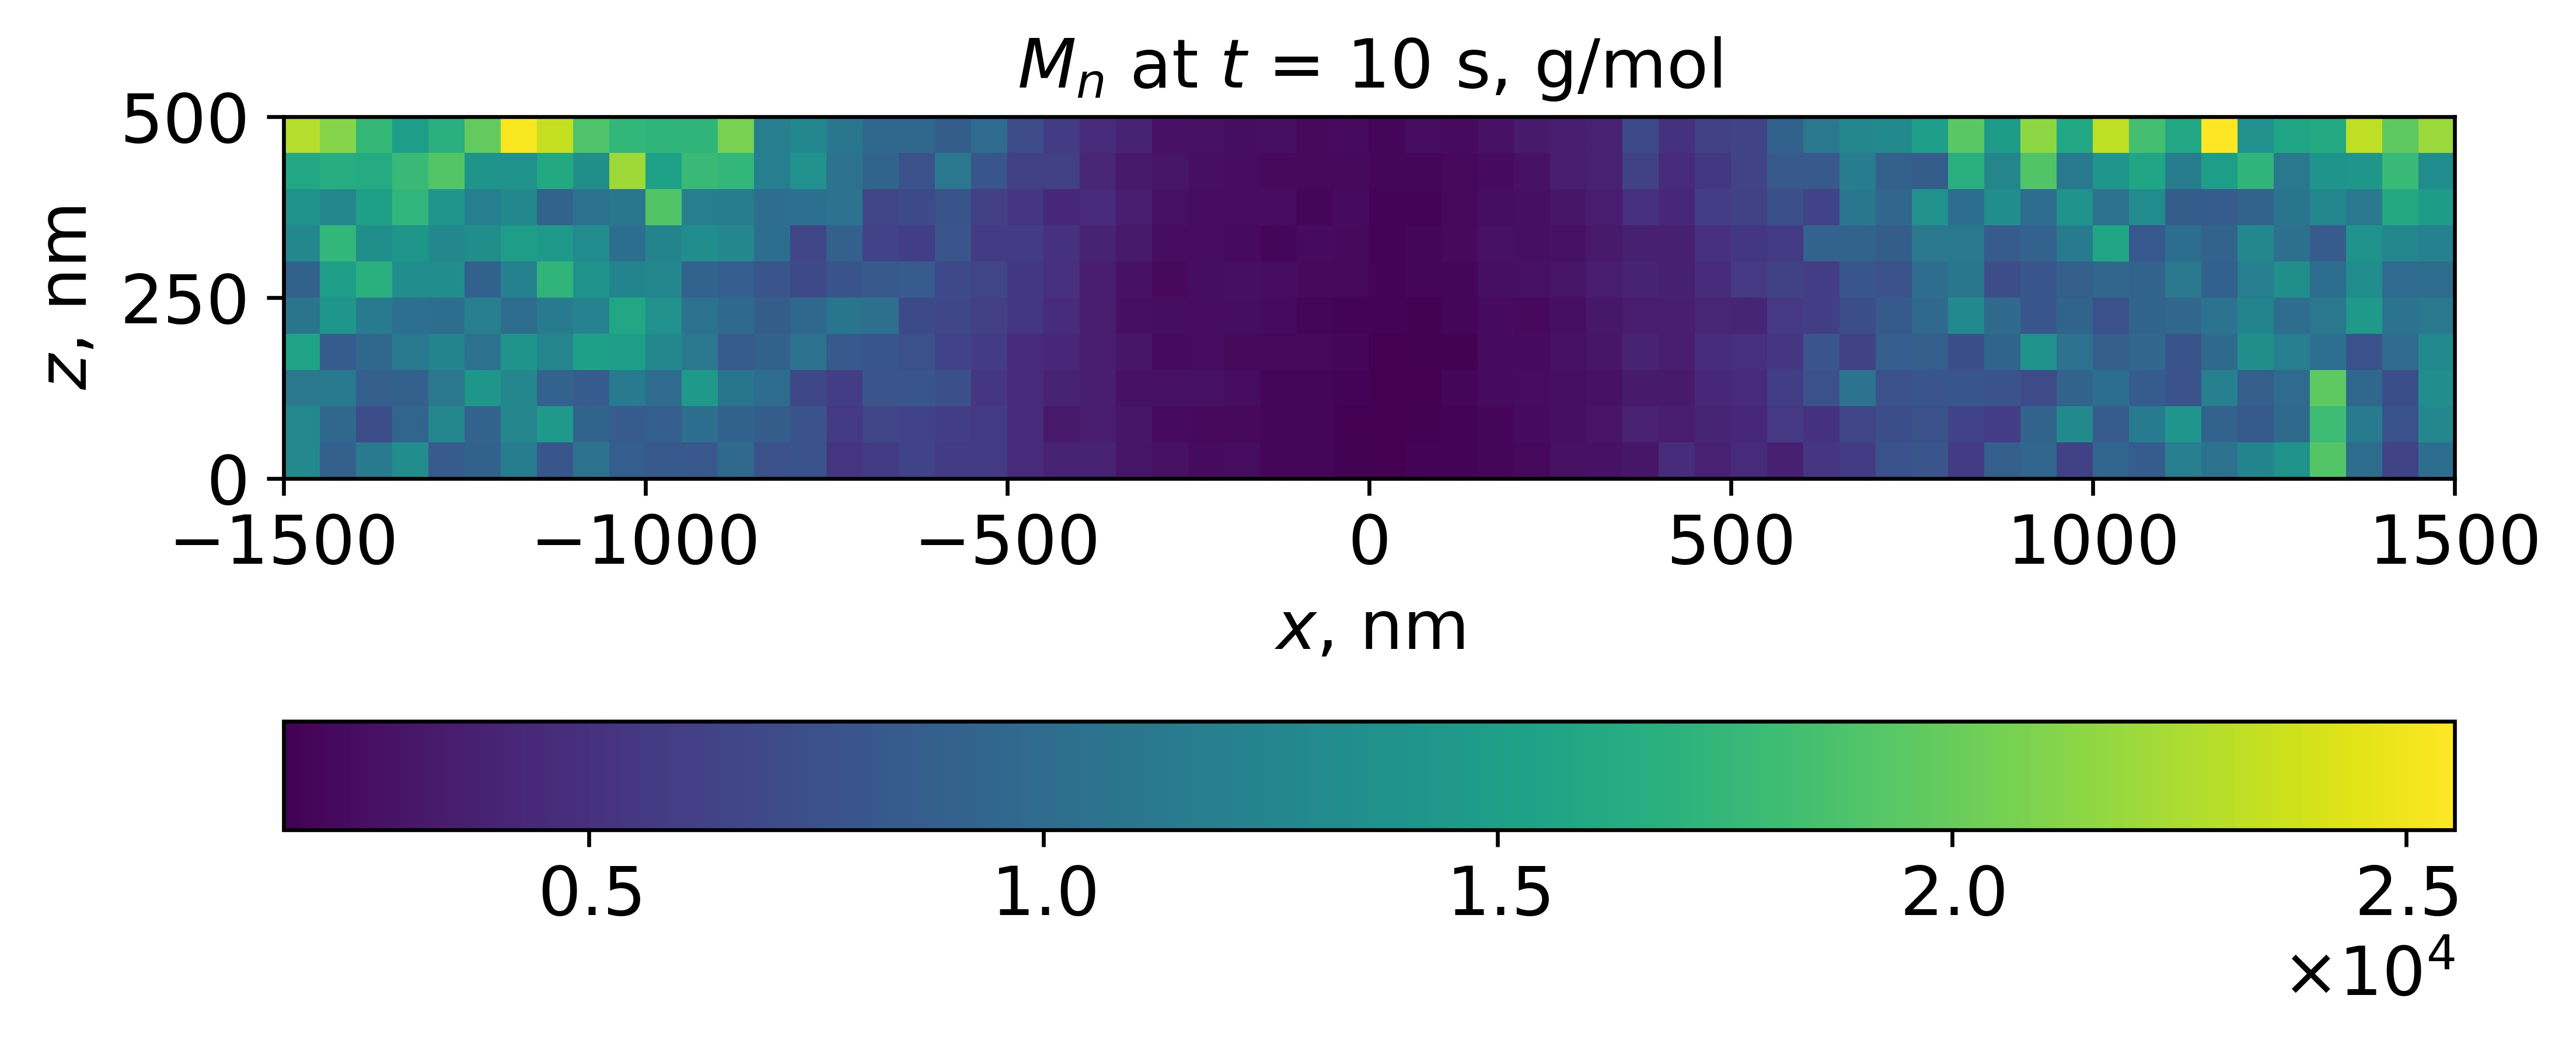
\includegraphics[width=0.7\linewidth]{Mn_hist_10s_14_eng} \\
		\vspace{-3.7em} \hspace{-26em} a) \vspace{2.7em} \\
		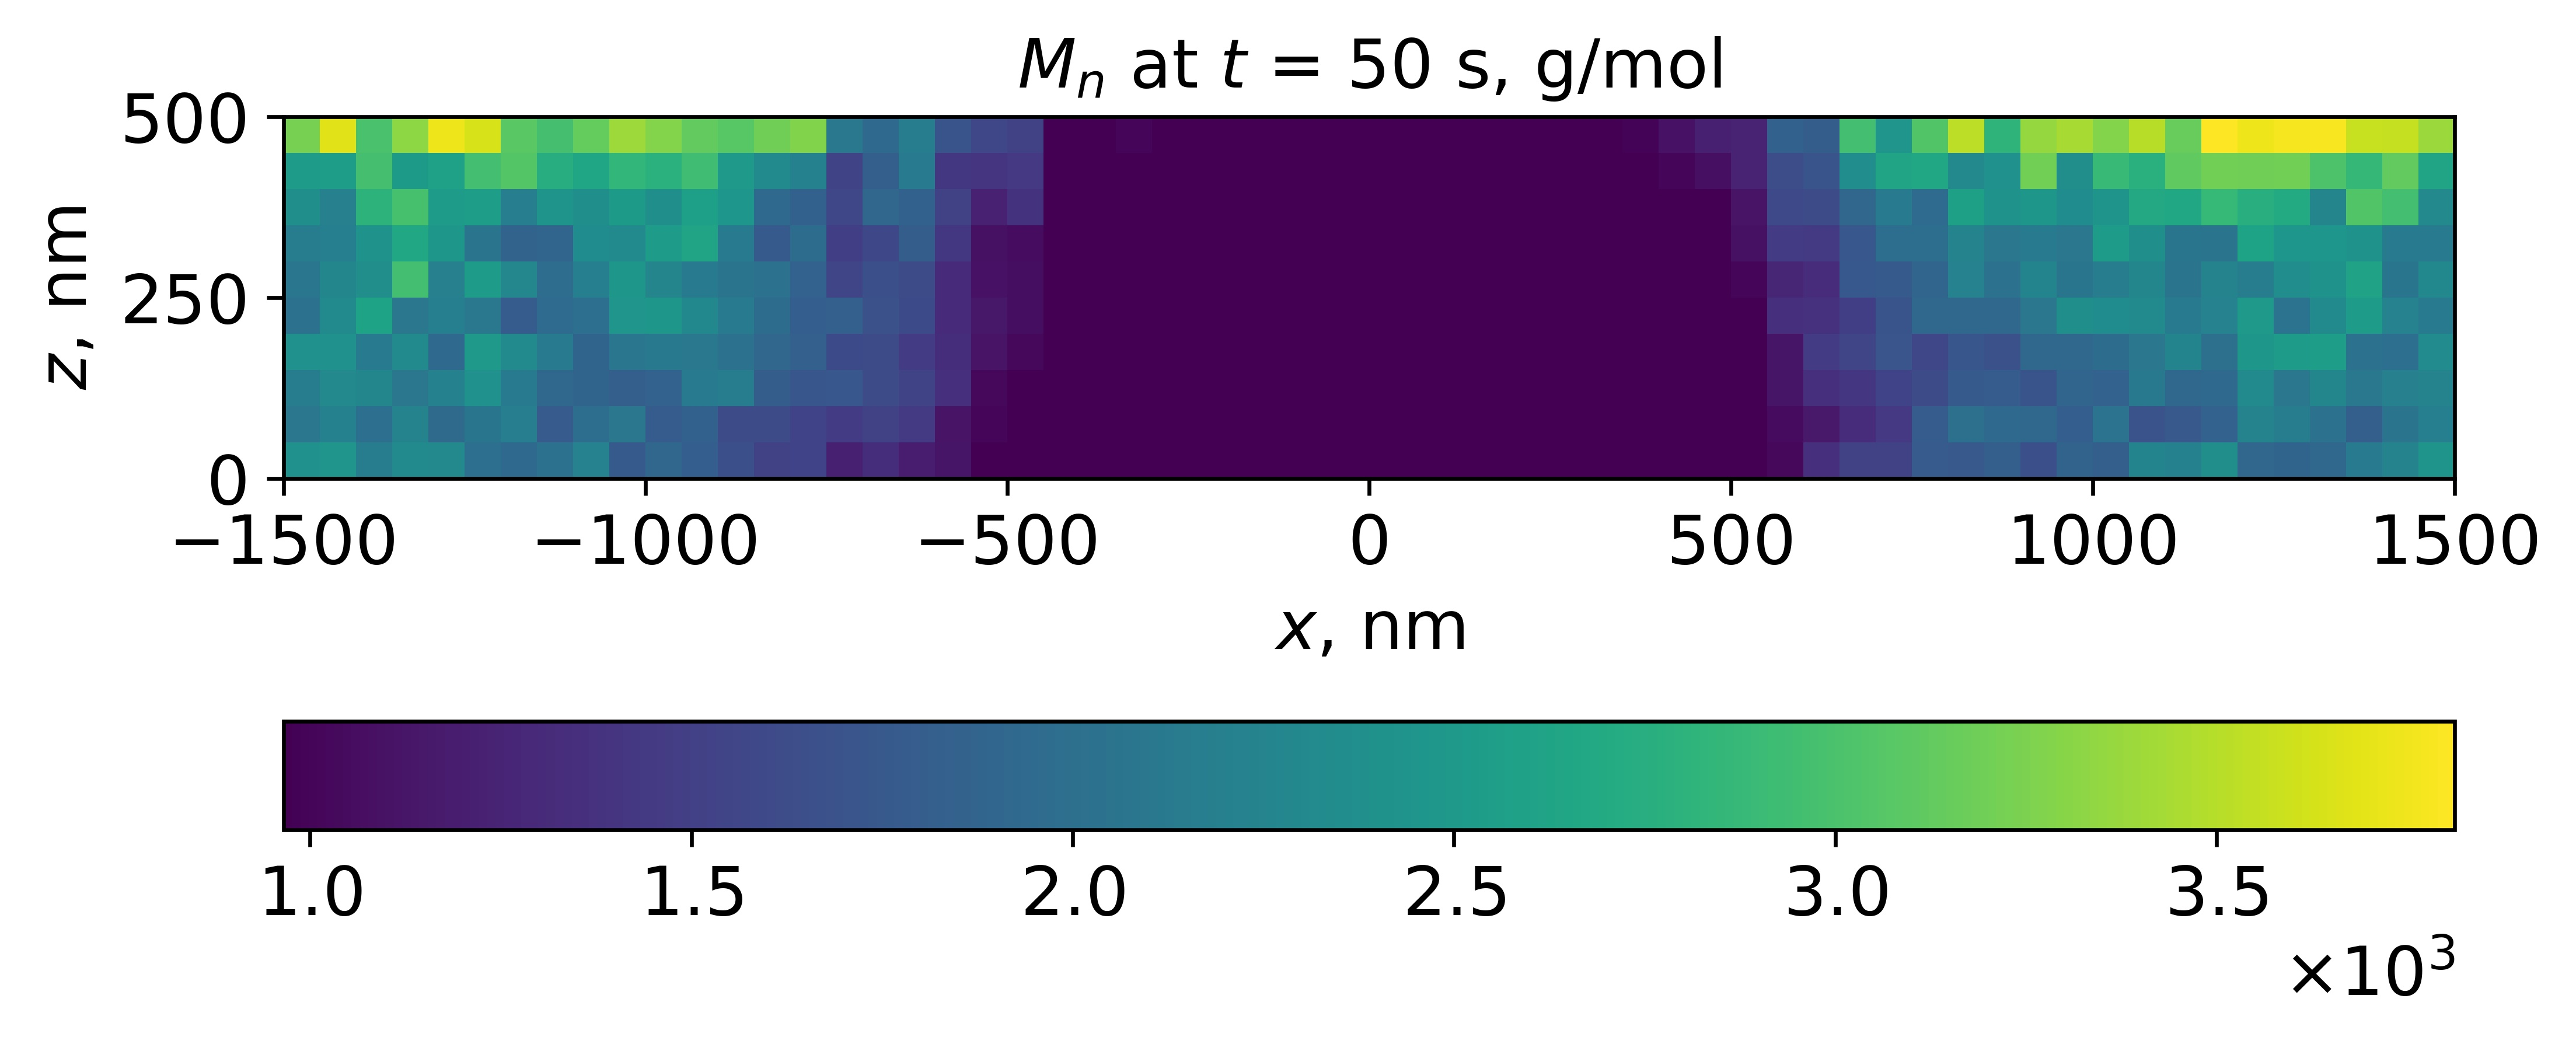
\includegraphics[width=0.7\linewidth]{Mn_hist_50s_14_eng} \\
		\vspace{-3.7em} \hspace{-26em} b) \vspace{3.7em} \\
	\end{center}
	\vspace{-2.5em}
	\caption{Simulation of PMMA molecular weight distribution during exposure in series of parallel lines. Line dose is around 3 nA/cm, e-beam energy is 20 keV, PMMA layer thickness -- 500 nm, exposure time is 10 s (a) and  50 s (b).}
	\label{fig:Mn_hist}
\end{figure}
